
            \documentclass[8pt]{beamer} 
            \usetheme{CambridgeUS} 
            \usepackage{textpos} 
            \usepackage[latin1]{inputenc} 
            \usepackage{amsmath} 
            \usepackage{mathtools} 
            \usepackage{color} 
            \usepackage{mathabx} 
            \usepackage{graphicx} 
            \usepackage{tikz} 
            \usepackage{esvect} 
            \usetikzlibrary{arrows,shapes} 
            \usecolortheme{beaver} 
            \usepackage{graphicx} 
            \usepackage{changepage} 
            \setbeamertemplate{navigation symbols}{} 
            \setbeamertemplate{navigation symbols}{} 
        
        \title{Example Document: How to use the LatexDocumentClass}
        \author{Riccardo Nicolaidis \footnote{mail@mail.mail}}
        \date{\today}
        
        \begin{document}
        
        \begin{frame}
            \titlepage
        \end{frame}
        
        \begin{frame}
            \frametitle{Introduction}
        
This is an example of how to use the LatexDocumentClass.

The LatexDocumentClass is a Python class that allows to create a Latex document in a very easy way.

It is built on top of the Latex Beamer class, and it is designed to create slides for presentations.

I created this class because it may be useful for managing output Report data from simulations, data analysis, etc.

You only need to do the following steps:

        \begin{itemize}
        
        \item Import the \texttt{LatexDocumentClass} class from the \texttt{LatexDocumentClass.py} file
        
        \item Instantiate the class
        
        \item Set name, author, title, email, output directory
        
        \item Build the body of the document by adding the desired content
        
        \item Compile the document
        
        \end{itemize}
        
        \end{frame}
        
        \begin{frame}
            \frametitle{Commands}
        
The following commands are available:

        \begin{itemize}
        
        \item \texttt{LatexDocument.BeginSlide(<Title of the slide>)}
        
        \item \texttt{LatexDocument.EndSlide()} (to be used at the end of the slide, if not the slide will not be closed and you'll get an error)
        
        \item \texttt{LatexDocument.BeginItemize()} (to be used at the beginning of an itemize environment)
        
        \item \texttt{LatexDocument.EndItemize()} (to be used at the end of an itemize environment, if not the itemize environment will not be closed and you'll get an error)
        
        \item \texttt{LatexDocument.Item(<Text of the item>)} (to be used inside an itemize environment, if not you'll get an error)
        
        \item \texttt{LatexDocument.Body} (to be used for adding text to the body of the document)
        
        \item \texttt{LatexDocument.InsertFigure(<Path of the image>, <Caption of the image>)} (to be used for adding a figure to the body of the document)
        
        \item \texttt{LatexDocument.Compile()} (For compiling and generating the PDF file)
        
        \end{itemize}
        
        \end{frame}
        
        \begin{frame}
            \frametitle{Example of a figure}
        
        \begin{figure}[h]
            \centering
            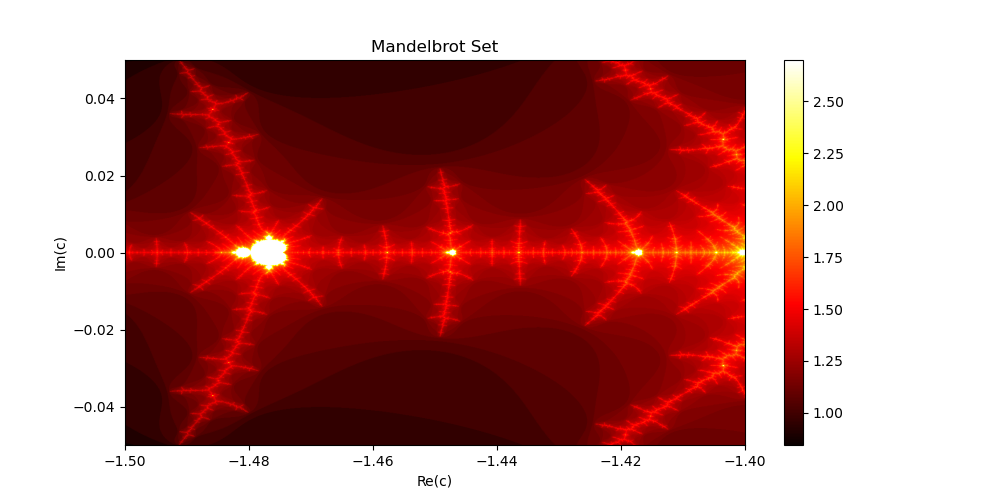
\includegraphics[width=1.0\textwidth]{/home/riccardo/Documenti/GeantProjects/LEM_GDML_upgrade/PythonMacros/Images/Test.png}
            \caption{A beautiful Mandelbrot Set}
        \end{figure}
        
        \end{frame}
        
        \begin{frame}
            \frametitle{Another interesting plot}
        
        \begin{figure}[h]
            \centering
            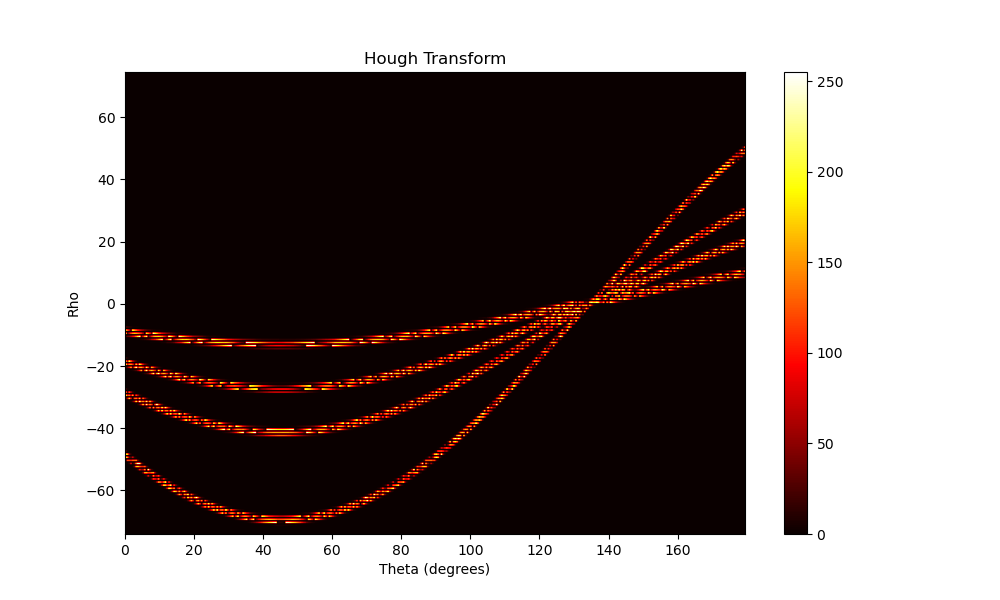
\includegraphics[width=1.0\textwidth]{/home/riccardo/Documenti/GeantProjects/LEM_GDML_upgrade/PythonMacros/Images/Test2.png}
            \caption{A beautiful Hough Transform}
        \end{figure}
        
        \end{frame}
        
        \begin{frame}
            \frametitle{End of the document}
        
This is the end of the document.

        \end{frame}
        
        \end{document}
        